\chapter{Magnetism}

\section*{LEARNING OUTCOMES}
{
\begin{center}
\fcolorbox{black}{shadecolor}{%

    \parbox{0.95\textwidth}
    {%
        \small
        {
        \begin{itemize}[leftmargin=*]\itemsep0em
            \item What are magnets?
            \item How many poles does a magnet have? How are they different?
            \item What objects do magnets attract and repel? How do they do it?
            \end{itemize}
        }
    }%
}
\end{center}
}

\section*{DEMONSTRATIONS}
\section*{Detection of Magnetic Field}
For this experiment, you will need:

\begin{table}[H]
    \centering
    \begin{tabular}{|c|l|c|}\hline
     \textbf{\#} & \textbf{Components}  &  \textbf{Amount}\\\hline
     1 & LED                            & 1\\\hline
     2 & 10 k$\Omega$ resistor           & 1\\\hline
     3 & 470 $\Omega$ resistor           & 1\\\hline
     4 & Buzzer                         & 1\\\hline
     5 & A3144: Hall effect sensor      & 1\\\hline
     6 & Permanent magnet               & 1\\\hline
     7 & Breadboard                     & 1\\\hline
     8 & Arduino UNO                    & 1\\\hline
     9 & Connecting wires               & - \\\hline
    \end{tabular}
\end{table}

\subsection*{Connections}
\begin{enumerate}[leftmargin=*]
    \item Connect the 5V and GND pins of Arduino board on the breadboard.
    \item Connect the Vcc and GND of the Hall effect sensor to the 5V and GND terminals respectively. 
    \item Connect a 10 k$\Omega$ resistor between the SIGNAL and Vcc pins of the module. Also connect the SIGNAL pin of the module to pin A$0$ of Arduino.
    \item Connect the anode of the LED to pin 9 through a $470~ \Omega$ resistor. Connect its cathode to GND.
    \item Connect the buzzer to pin 9 and GND.
    
\end{enumerate}

\begin{figure}[H]
    \centering
    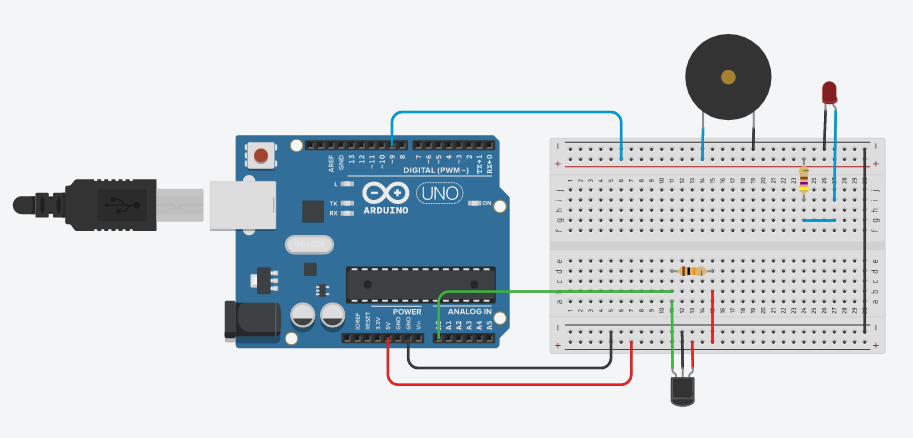
\includegraphics[scale=0.5]{Figures/magnetism.PNG}
    \caption{Circuit diagram}
\end{figure}

\subsection*{Procedure}
\begin{enumerate}[leftmargin=*]
    \item Copy lst. \ref{lst:magnet} to a new Arduino sketchbook. Upload the code to Arduino UNO. Also open the Serial Monitor.
    \item Bring the north pole of the permanent magnet near the Hall effect module. Observe the change in the states of the LED and the buzzer.
    \item Change the pole of the magnet and repeat the experiment. Observe the change in the states of the LED and the buzzer.
    \item Repeat the previous steps by bringing the magnet near the opposite side of the Hall effect sensor.
\end{enumerate}
%Arduino Code
\begin{lstlisting}[language=Arduino, numbers=none, caption={Arduino code for measuring the intensity of light measured by LDR}, captionpos=b, label={lst:magnet}]

int magnet=A0;
int out = 9;

void setup() 
{
  // put your setup code here, to run once:
  pinMode(magnet, INPUT);    // A0 is declared an input peripheral
  pinMode(out, OUTPUT); 
  Serial.begin(9600);
}

void loop() 
{
  // put your main code here, to run repeatedly:
  
  int intensity = analogRead(magnet);    
  // The magnetic field intensity is recorded
  
  Serial.println(intensity);          
  // The field intensity is printed either on Serial Monitor or on Serial Plotter
  
  analogWrite(out, intensity/4);
        
  delay(50);                      //Add a delay of 50 ms
}

\end{lstlisting}

\begin{figure}[H]
    \centering
    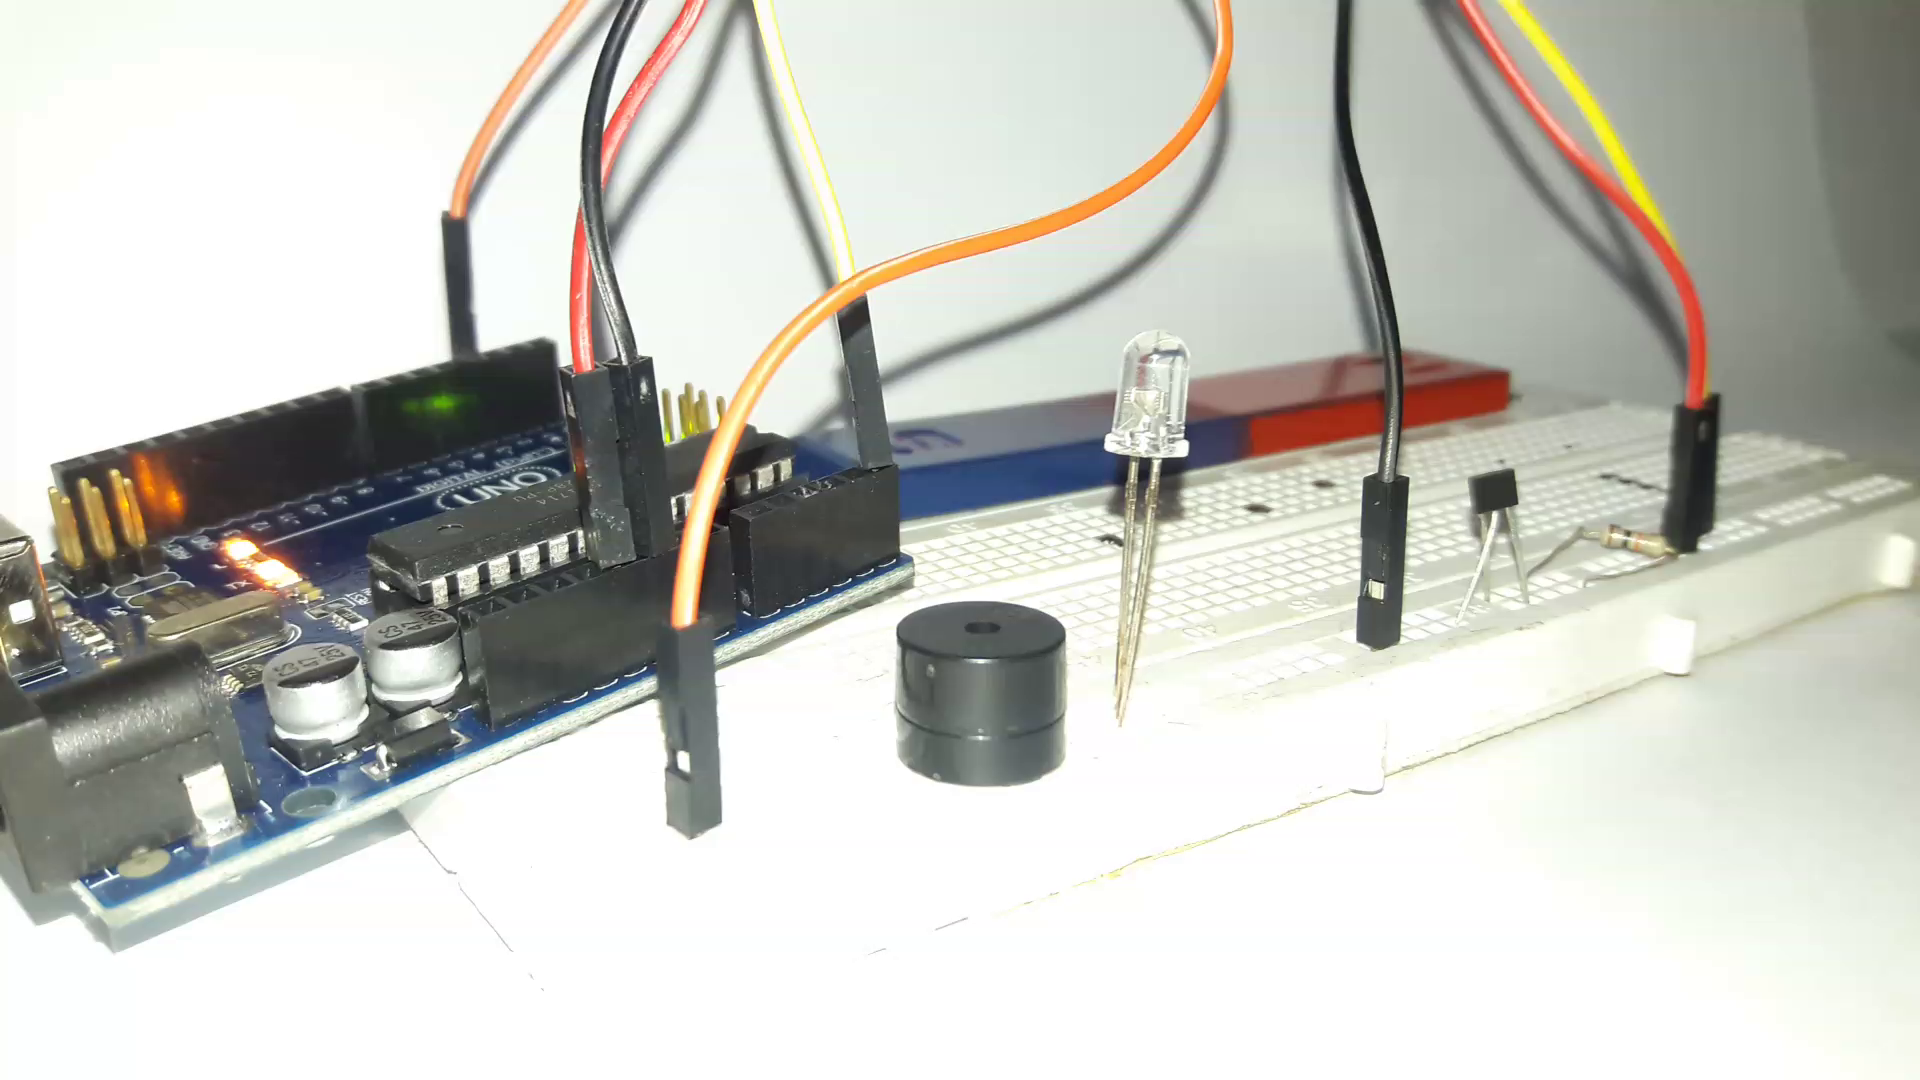
\includegraphics[width=0.75\linewidth]{Figures/magnetism-hardware.png}
    \caption{Hardware of the experiment}
    \label{fig:my_label}
\end{figure}
